\chapter{Phá vỡ đối xứng, boson Goldstone và bất biến chuẩn}

Chúng ta muốn hiểu làm thế nào một hạt giống photon có thể có được khối lượng. Đó là đích đến, nhưng không phải là điểm xuất phát hợp lý. Một hạng khối lượng trực tiếp cho một trường chuẩn dường như phá hủy chính tính bất biến chuẩn làm cho lý thuyết nhất quán. Trước khi có thể thấy lối thoát, ta cần 2 ý tưởng ở dạng đủ cụ thể để làm việc:
\begin{enumerate}
  \item sự phá vỡ đối xứng tự phát, đặc biệt đối với một đối xứng liên tục;
  \item bất biến chuẩn, trong đó phép đối xứng có thể thay đổi từ điểm không-thời gian này sang điểm không-thời gian khác.
\end{enumerate}
Không ý tưởng nào trong hai có thể được thay bằng một khẩu hiệu. Ta sẽ xây dựng ý tưởng thứ nhất từ một nam châm, chuyển nó sang lý thuyết trường vô hướng, và phát hiện mode Goldstone không khối lượng. Sau đó ta sẽ lấy chính đối xứng \(U(1)\) ấy và làm cho nó trở thành cục bộ, điều buộc ta phải đưa vào một thế vectơ và một đạo hàm hiệp biến. Chỉ đến cuối, 2 mạch này mới được đặt cạnh nhau. Sự hợp nhất thực sự của chúng---hiện tượng Higgs---là chủ đề của bài giảng tiếp theo.

\section{Một định luật đối xứng với trạng thái cơ bản bất đối xứng}

\subsection{Nam châm hai trạng thái}

Hãy bắt đầu với một mạng gồm các nam châm nhỏ. Mỗi spin có thể hướng lên hoặc xuống, và các spin lân cận làm giảm năng lượng của chúng bằng cách cùng chỉ theo một hướng. Trên một mạng lập phương 3 chiều, một spin có 6 láng giềng gần nhất, nhưng số phối trí chính xác không quan trọng. Điều quan trọng là quy tắc
\begin{equation}
  E_{\parallel}<E_{\rm antiparallel}.
\end{equation}
Quy tắc vi mô không thay đổi nếu đảo ngược mọi spin:
\begin{equation}
  \uparrow\longleftrightarrow\downarrow.
\end{equation}
Tuy nhiên, các cấu hình năng lượng thấp nhất tự chúng không đối xứng. Chúng là
\begin{equation}
  \{\uparrow\uparrow\uparrow\cdots\},
  \qquad
  \{\downarrow\downarrow\downarrow\cdots\}.
\end{equation}
Các phương trình cho phép cả hai, nhưng một mẫu vĩ mô lạnh buộc phải chọn một.

Sự lựa chọn này nhạy cảm đến phi thường. Hãy cố định một spin ở rất xa sao cho nó hướng lên. Các láng giềng của nó thích làm theo nó, các láng giềng của chúng lại thích làm theo chúng, và thông tin ấy lan truyền xuyên qua mẫu. Một nhiễu loạn nhỏ tùy ý so với toàn bộ hệ có thể chọn định hướng của toàn bộ trạng thái cơ bản. Đó là tính bất ổn được hàm ý bởi sự phá vỡ đối xứng \emph{tự phát}.

\begin{classroomqa}
\audiencequestion{Một hạt trung hòa có thể tự định hướng trong từ trường không?
\lecturetimestamp{00:05:14}}
\lecturerresponse{Có. Tính trung hòa điện không hàm ý sự vắng mặt của mômen từ. Neutron là trung hòa nhưng có mômen từ do các thành phần mang điện bên trong nó. Vì thế, một từ trường có thể phân biệt các định hướng spin của nó.}
\end{classroomqa}

\begin{classroomqa}
\audiencequestion{Nếu hệ đổi định hướng, sự thay đổi có xảy ra đồng thời ở mọi nơi không? Có thể có nhiều sóng tái định hướng cùng tồn tại không?
\lecturetimestamp{00:05:41--00:06:38}}
\lecturerresponse{Sự thay đổi lan truyền. Một vùng làm các vùng lân cận nghiêng theo nó, khá giống một dãy quân domino 3 chiều, và nhiễu loạn truyền đi như một làn sóng. Các vùng khác nhau có thể bắt đầu lựa chọn một cách độc lập, nên có thể hiện diện nhiều mặt trước và nhiều miền trước khi một định hướng thắng thế. Chúng ta sẽ quay lại chính những sóng này khi đối xứng trở thành liên tục.}
\end{classroomqa}

\subsection{Phá vỡ tường minh là một lý thuyết khác}

Bây giờ đặt mẫu trong một từ trường ngoài hướng lên trên. Một spin cô lập đã có năng lượng thấp hơn khi nó hướng lên. Phép biến đổi \(\uparrow\leftrightarrow\downarrow\) không còn giữ nguyên năng lượng nữa: sự ưu tiên đã được cài ngay vào bản thân định luật. Đây là sự phá vỡ đối xứng \emph{tường minh}.

Có thể kiểm tra sự khác biệt này mà không cần biết mẫu đã được chuẩn bị như thế nào. Lấy một mẫu rất lớn, giữ biên trái của nó hướng lên, và giữ biên phải của nó hướng xuống. Nếu một từ trường trong khối ưu tiên tường minh hướng lên, thì ràng buộc ở phía phải chỉ xâm nhập được một quãng ngắn. Một vùng xuống vĩ mô sẽ phải trả một năng lượng tỉ lệ với thể tích của nó, nên phần khối không thể duy trì sự phân chia thành 2 pha thuận lợi như nhau.

Nếu không có thiên lệch bên ngoài, hướng lên và hướng xuống có cùng năng lượng trong khối. Khi đó trạng thái bị ràng buộc có năng lượng thấp nhất chứa một miền hướng lên, một miền hướng xuống, và một lớp chuyển tiếp hữu hạn giữa chúng. Mặt phân cách không nhất thiết phải nằm ở tâm hình học, nhưng không có áp lực theo thể tích nào buộc một pha phải xóa bỏ pha kia. Mặt phân cách này là một \emph{vách miền}, khuyết tật đặc trưng của đối xứng rời rạc bị phá vỡ này.

\begin{figure}[htbp]
\centering
\begin{adjustbox}{max width=\linewidth}
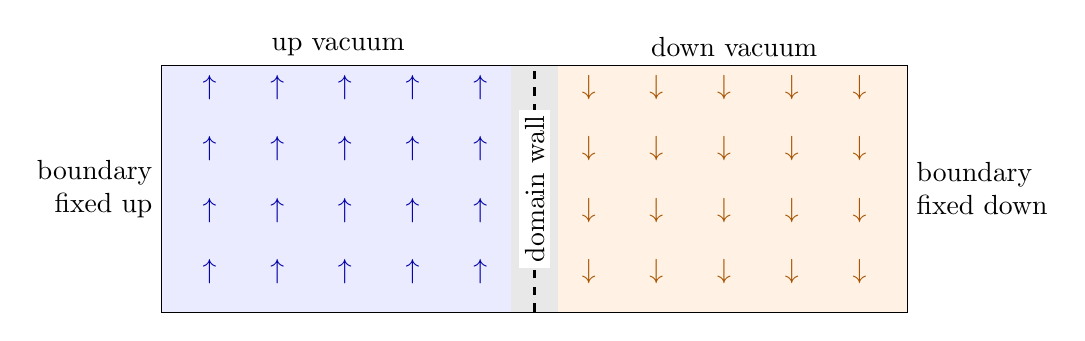
\begin{tikzpicture}[x=0.86cm,y=0.78cm]
  \draw[thick] (0,0) rectangle (11,4);
  \fill[blue!8] (0,0) rectangle (5.15,4);
  \fill[orange!10] (5.85,0) rectangle (11,4);
  \fill[gray!18] (5.15,0) rectangle (5.85,4);
  \foreach \x in {0.7,1.7,2.7,3.7,4.7}
    \foreach \y in {0.65,1.65,2.65,3.65}
      \node[blue!65!black] at (\x,\y) {$\uparrow$};
  \foreach \x in {6.3,7.3,8.3,9.3,10.3}
    \foreach \y in {0.65,1.65,2.65,3.65}
      \node[orange!65!black] at (\x,\y) {$\downarrow$};
  \draw[dashed,thick] (5.5,0) -- (5.5,4);
  \node[above] at (2.6,4) {up vacuum};
  \node[above] at (8.45,4) {down vacuum};
  \node[rotate=90,fill=white,inner sep=2pt] at (5.5,2) {domain wall};
  \node[left,align=right] at (0,2) {boundary\\fixed up};
  \node[right,align=left] at (11,2) {boundary\\fixed down};
\end{tikzpicture}
\end{adjustbox}
\caption{Phép kiểm tra bằng điều kiện biên đối với sự phá vỡ tự phát của một đối xứng rời rạc. Hai định hướng trong khối có cùng năng lượng, nên một vách có thể ngăn cách các miền vĩ mô.}
\end{figure}

\begin{classroomqa}
\audiencequestion{Lập luận này có đòi hỏi tương tác chỉ giữa các láng giềng gần nhất không?\lecturetimestamp{00:18:18}}
\lecturerresponse{Không. Một tương tác với láng giềng thứ hai cũng ưu tiên sự thẳng hàng sẽ làm thay đổi chi tiết nhưng không thay đổi kết luận. Hành vi thú vị hơn xuất hiện nếu các tầm tương tác khác nhau cạnh tranh nhau---chẳng hạn, các láng giềng gần nhất thích thẳng hàng còn các láng giềng gần kế tiếp lại thích phản thẳng hàng. Điều đó tạo ra frustration và các pha có trật tự phức tạp hơn, nhưng không làm thay đổi sự phân biệt cơ bản đang được nêu ra ở đây.}
\end{classroomqa}

\begin{classroomqa}
\audiencequestion{Từ \emph{tự phát} có ám chỉ đạo hàm lớn ở bên trong vách không?\lecturetimestamp{00:19:05}}
\lecturerresponse{Không. Nó ám chỉ thực tế rằng năng lượng nền tảng không hề ưu tiên hướng lên--xuống, trong khi trạng thái cơ bản được chọn thì có. Sự đáp ứng mạnh trước một nhiễu loạn nhỏ tùy ý cho thấy một tính bất ổn. Gradient chỉ đơn thuần cho biết mặt phân cách tốn bao nhiêu năng lượng.}
\end{classroomqa}

\begin{classroomqa}
\audiencequestion{Vật liệu vốn đã ở một trong 2 trạng thái ấy, hay trạng thái của nó ban đầu chưa được biết?\lecturetimestamp{00:19:40}}
\lecturerresponse{Điều đó phụ thuộc vào lịch sử của nó. Ở nhiệt độ cao, chuyển động nhiệt có thể để các spin lên và xuống trộn lẫn với độ từ hóa trung bình gần bằng 0. Khi vật liệu nguội đi, các vùng nhỏ chọn những định hướng khác nhau, các vách miền hình thành, và các miền lớn dần lên. Ngẫu nhiên và các nhiễu loạn môi trường cực nhỏ quyết định chân không nào rốt cuộc chiếm phần lớn mẫu.}
\end{classroomqa}

\section{Cùng lập luận đó trong lý thuyết trường vô hướng}

Thay các spin bằng một trường vô hướng thực \(\phi(\bm{x},t)\). Với các quy ước về metric và chuẩn hoá đã được ấn định một lần dứt khoát, viết
\begin{equation}
\begin{aligned}
  \mathcal L
  &=\frac12\,\partial_\mu\phi\,\partial^\mu\phi-V(\phi),
  \\
  \mathcal E
  &=\frac12\dot\phi^{\,2}+\frac12(\nabla\phi)^2+V(\phi).
\end{aligned}
  \label{eq:l07-real-scalar}
\end{equation}
Ký pháp tương đối tính rút gọn trong \(\mathcal L\) chứa hạng đạo hàm theo thời gian dương và hạng gradient không gian âm; còn mật độ năng lượng Hamiltonian thì cả hai đóng góp đều dương.

Hãy chọn một thế chẵn với 2 cực tiểu suy biến,
\begin{equation}
  V(\phi)=\frac{\lambda}{4}\left(\phi^2-f^2\right)^2,
  \qquad \lambda>0.
  \label{eq:l07-double-well}
\end{equation}
Lagrangian bất biến dưới phép \(\phi\mapsto-\phi\), còn một trong hai chân không đồng đều
\begin{equation}
  \phi(\bm{x})=+f,
  \qquad\hbox{or}\qquad
  \phi(\bm{x})=-f
\end{equation}
lại chọn một phía. Ngược lại, một thế chỉ có một cực tiểu duy nhất tại \(\phi=0\) có chân không đối xứng và không bị phá vỡ đối xứng tự phát.

Hãy cố định \(\phi=+f\) ở một phía của mẫu và \(\phi=-f\) ở phía kia. Trường không thể nhảy đột ngột mà không phải trả giá, vì
\begin{equation}
  E_{\rm wall}
  =\int dx\left[
      \frac12\left(\frac{d\phi}{dx}\right)^2+V(\phi)-V(f)
    \right].
  \label{eq:l07-wall-energy}
\end{equation}
Một bước nhảy đột ngột làm \(d\phi/dx\) trở nên cực lớn. Vì thế, vách có năng lượng cực tiểu sẽ dàn sự thay đổi ra trên một bề rộng hữu hạn, cân bằng năng lượng gradient với cái giá về thế khi đi qua vùng giữa các cực tiểu. Nghiệm kink quen thuộc cho thế trong phương trình ~\eqref{eq:l07-double-well} là
\begin{equation}
  \phi_{\rm wall}(x)
  =f\tanh\!\left[f\sqrt{\frac{\lambda}{2}}\,(x-x_0)\right],
  \label{eq:l07-kink}
\end{equation}
một hiện thực hóa tường minh của chuyển tiếp trơn đã được mô tả trên bảng.
\editorialnote{Bài giảng lập luận từ hình dạng của thế và hạng gradient nhưng không giải phương trình trường. Phương trình
\eqref{eq:l07-kink} được đưa vào như nghiệm chuẩn của mô hình đã nêu, làm cho bức tường định tính trở nên cụ thể mà không thay đổi lập luận.}

Hãy làm nghiêng nhẹ thế hai giếng, khi đó một cực tiểu trở nên thấp hơn. Khi ấy chính Lagrangian là bất đối xứng. Một vách vẫn có thể xuất hiện tạm thời, nhưng chân không năng lượng cao hơn, hay chân không giả, tác dụng một áp lực lên nó; vách chuyển động và pha được ưu tiên giãn nở ra. Đây là phiên bản trong lý thuyết trường của sự phá vỡ tường minh do một từ trường ngoài.

Cho đến đây, đối xứng là rời rạc. Vật lý hạt bị chi phối bởi các nhóm liên tục như \(U(1)\), \(SU(2)\) và \(SU(3)\). Một đối xứng liên tục làm thay đổi bức tranh về khuyết tật và đưa vào một loại hạt mới.

\section{Một trường phức và \texorpdfstring{\(U(1)\)}{U(1)} toàn cục}

\subsection{Các phép quay trong một mặt phẳng nội tại}

Hãy đặt
\begin{equation}
  \phi=\phi_R+i\phi_I,
  \qquad
  \phi^*=\phi_R-i\phi_I,
  \qquad
  \phi^*\phi=\phi_R^2+\phi_I^2.
  \label{eq:l07-components}
\end{equation}
Các trục \(\phi_R\) và \(\phi_I\) tạo thành một không gian trường nội tại, chứ không phải 2 phương trong không gian thông thường. Một vô hướng phức đơn giản chỉ là 2 trường vô hướng thực được gói lại sao cho các phép quay trong mặt phẳng nội tại này hiện ra tường minh.

\begin{figure}[htbp]
\centering
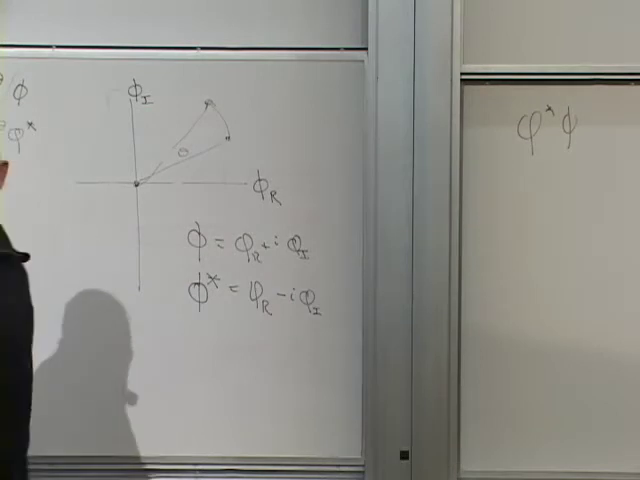
\includegraphics[width=0.80\textwidth]{lecture_07_figure_02.png}
\caption{Trường phức trên mặt phẳng nội tại \((\phi_R,\phi_I)\). Trên bảng ghi phép phân tích của \(\phi\) và \(\phi^*\) cùng bán kính bất biến \(\phi^*\phi\).}
\lectureframe{00:33:33}
\end{figure}

Sử dụng Lagrangian
\begin{equation}
  \mathcal L
  =\partial_\mu\phi^*\,\partial^\mu\phi
   -V(\phi^*\phi).
  \label{eq:l07-complex-lagrangian}
\end{equation}
Đối với trường phức, thừa số thông thường \(1/2\) không có mặt, vì riêng tích này đã chứa các hạng động học của cả hai thành phần thực.
Phép biến đổi
\begin{equation}
  \phi'(x)=e^{i\theta}\phi(x),
  \qquad
  \phi^{*\prime}(x)=e^{-i\theta}\phi^*(x)
  \label{eq:l07-global-u1}
\end{equation}
quay mọi giá trị của trường một góc như nhau. Ở đây \(\theta\) là hằng số theo không gian và thời gian. Dấu phẩy trên ký hiệu chỉ trường sau biến đổi; đó không phải là đạo hàm.

Vì \(\theta\) là hằng,
\begin{equation}
  \partial_\mu\phi'=e^{i\theta}\partial_\mu\phi,
  \qquad
  \partial_\mu\phi^{*\prime}
  =e^{-i\theta}\partial_\mu\phi^*.
\end{equation}
Các pha triệt tiêu nhau trong hạng động năng, và \(\phi^{*\prime}\phi'=\phi^*\phi\). Vì vậy, mọi thế chỉ phụ thuộc vào \(\phi^*\phi\) đều có cùng đối xứng ấy. Một hạng chỉ phụ thuộc riêng vào \(\phi_R\) sẽ chọn một hướng trong mặt phẳng nội tại và phá vỡ nó một cách tường minh.

\subsection{Một cực tiểu tại một điểm và một đường tròn các cực tiểu}

Có 2 loại thế đối xứng khác nhau về mặt định tính. Loại thứ nhất chỉ có cực tiểu duy nhất tại gốc, chẳng hạn
\begin{equation}
  V_{\rm unbroken}=m^2\phi^*\phi,
  \qquad m^2>0.
\end{equation}
Đồ thị của nó là một paraboloid đối xứng quay. Chân không \(\phi=0\) đứng yên dưới mọi phép quay, nên đối xứng là không bị phá vỡ.

Bây giờ hãy chọn
\begin{equation}
  V_{\rm broken}
  =-a\,\phi^*\phi+b(\phi^*\phi)^2,
  \qquad a,b>0.
  \label{eq:l07-mexican-hat}
\end{equation}
Hạng bậc hai âm đẩy trường ra xa gốc, còn hạng bậc bốn dương ngăn nó chạy ra vô cùng. Viết
\(r^2=\phi^*\phi\), việc cực tiểu hóa cho
\begin{equation}
  \frac{dV}{d(r^2)}=-a+2br^2=0,
  \qquad
  r^2=f^2=\frac{a}{2b}.
  \label{eq:l07-vacuum-radius}
\end{equation}
Vì thế, các cực tiểu tạo thành một đường tròn. Thế hoàn toàn đối xứng quay, nhưng một trạng thái cơ bản đồng đều buộc phải chọn một điểm trên đường tròn ấy.

\begin{figure}[htbp]
\centering
\includegraphics[width=0.72\textwidth]{lecture_07_figure_06.png}
\caption{Thế phá vỡ đối xứng được vẽ như một mặt tròn xoay. Gốc tọa độ là bất ổn và các cực tiểu suy biến tạo thành rãnh tròn.}
\lectureframe{00:37:25}
\end{figure}

Hãy hình dung trường như một mũi tên nhỏ trong mặt phẳng nội tại này tại mỗi điểm của không gian thông thường. Thế yêu cầu mọi mũi tên đều có độ dài \(f\). Năng lượng gradient yêu cầu các mũi tên lân cận chỉ gần như cùng một hướng. Vì vậy, trạng thái cơ bản có cùng một góc ở mọi nơi, nhưng không góc nào được định luật ưu tiên. Đó là sự phá vỡ tự phát của một đối xứng liên tục.

\section{Từ vách miền đến một xoắn trơn}

Hãy lặp lại thí nghiệm điều kiện biên. Ở biên trái, cố định trường tại một điểm chân không \(A\); ở biên phải, cố định nó tại một điểm chân không khác \(B\). Một bước nhảy cục bộ sẽ làm gradient lớn. Tuy nhiên, khác với trường hợp rời rạc, trường có thể vẫn nằm ở đáy của thế trong khi thay đổi liên tục quanh đường tròn.

Ở năng lượng thấp, viết trường thành \(\phi=f e^{i\alpha(x)}\). Trong 1 chiều không gian, năng lượng liên quan là
\begin{equation}
  E[\alpha]
  =f^2\int_0^L dx\,\left(\frac{d\alpha}{dx}\right)^2.
  \label{eq:l07-angle-functional}
\end{equation}
Với các góc ở hai đầu mút được cố định, phép biến phân cho
\begin{equation}
  \frac{d^2\alpha}{dx^2}=0,
  \qquad
  \alpha(x)=\alpha_A+
    \frac{\alpha_B-\alpha_A}{L}\,x.
  \label{eq:l07-linear-twist}
\end{equation}
Cấu hình được ưu tiên dàn đều độ xoắn trên toàn bộ mẫu. Năng lượng của nó tỉ lệ như
\begin{equation}
  E_{\rm twist}
  =f^2\frac{(\alpha_B-\alpha_A)^2}{L},
  \label{eq:l07-twist-energy}
\end{equation}
nên có thể làm cho nó rẻ tùy ý bằng cách tăng \(L\).

\begin{figure}[htbp]
\centering
\begin{adjustbox}{max width=\linewidth}
\begin{tikzpicture}[x=0.95cm,y=0.95cm]
  \begin{scope}
    \draw[->] (0,0) -- (6.2,0) node[right] {$x$};
    \draw[->] (0,0) -- (0,3.5) node[above] {$\alpha(x)$};
    \draw[very thick,blue!70!black] (0.45,0.65) -- (5.7,2.85);
    \fill (0.45,0.65) circle (1.8pt) node[left] {$\alpha_A$};
    \fill (5.7,2.85) circle (1.8pt) node[right] {$\alpha_B$};
    \node at (3.1,-0.65) {physical space};
  \end{scope}
  \begin{scope}[xshift=9.2cm,yshift=1.65cm]
    \draw[thick] (0,0) circle (1.8);
    \fill (1.55,-0.92) circle (1.8pt) node[below right] {$A$};
    \fill (-0.45,1.74) circle (1.8pt) node[above] {$B$};
    \draw[very thick,blue!70!black,-{Latex[length=2.5mm]}]
      (1.55,-0.92) arc[start angle=-31,end angle=104,radius=1.8];
    \node at (0,-2.35) {vacuum circle};
  \end{scope}
\end{tikzpicture}
\end{adjustbox}
\caption{Cùng một cấu hình năng lượng thấp trong 2 cách mô tả. Góc biến thiên tuyến tính theo không gian vật lý, trong khi trường đi theo cung ngắn của đường tròn chân không trong không gian nội tại.}
\end{figure}

\begin{classroomqa}
\audiencequestion{Có thể có hai cách đi quanh đường tròn. Trường đi theo lộ trình nào, và nó có thể bị mắc kẹt trên lộ trình dài hơn không?
\lecturetimestamp{00:41:54}}
\lecturerresponse{Với các điểm cuối tổng quát, lộ trình góc ngắn hơn có gradient nhỏ hơn và do đó năng lượng thấp hơn. Các điểm cuối đối diện nhau qua đường kính làm cho hai lộ trình đơn giản nhất suy biến. Một cấu hình được chuẩn bị bằng cách di chuyển chậm một điểm cuối có thể giữ lại một số quấn bổ sung và bị mắc kẹt sau một rào cản năng lượng, nhưng với một cặp điểm cuối thông thường đã cho thì lộ trình ngắn nhất không xoắn là trạng thái cơ bản.}
\end{classroomqa}

\begin{classroomqa}
\audiencequestion{Liệu một lộ trình có thể rời đáy rãnh và cắt ngang qua phần bên trong để trở nên ngắn hơn về tổng thể không?\lecturetimestamp{00:43:32}}
\lecturerresponse{Trong chế độ năng lượng thấp và mẫu dài, việc leo lên thế năng theo bán kính là không đáng. Giữ bán kính ở giá trị chân không của nó và cho góc biến thiên tuyến tính sẽ cực tiểu hóa năng lượng hiệu dụng, như phép tính giải tích biến phân ở trên cho thấy. Đối với một hệ hữu hạn với một thế năng cụ thể, ta có thể cực tiểu hóa đồng thời chuyển động theo bán kính và theo góc, nhưng kết luận Goldstone liên quan đến giới hạn bước sóng dài tùy ý, trong đó chuyển động trơn dọc theo rãnh thắng thế.}
\end{classroomqa}

\begin{classroomqa}
\audiencequestion{Điều gì thay đổi nếu rãnh tròn bị nghiêng đi sao cho một góc có năng lượng thấp hơn?\lecturetimestamp{00:44:33}}
\lecturerresponse{Khi đó đối xứng bị phá vỡ tường minh. Một điểm trở thành trạng thái cơ bản thực sự, chuyển động dọc theo đường tròn có lực hồi phục, và kích thích góc không còn chính xác là không khối lượng.}
\end{classroomqa}

\section{Khối lượng như cái giá của một dao động có xung lượng bằng không}

Sự xoắn trơn bộc lộ một trường mà năng lượng chỉ đến từ các gradient. Để hiểu vì sao điều đó có nghĩa là một hạt không khối lượng, hãy so sánh với hệ thức tán sắc tương đối tính
\begin{equation}
  \omega^2=\bm{k}^2+m^2.
  \label{eq:l07-dispersion}
\end{equation}
Một sóng \(e^{i(\bm{k}\cdot\bm{x}-\omega t)}\) mang xung lượng \(\bm{k}\).
Nếu \(m=0\), năng lượng của nó tiến về 0 khi bước sóng tiến tới vô hạn:
\(\omega=|\bm{k}|\to0\). Nếu \(m\ne0\), một mode đồng nhất theo không gian
\(\bm{k}=0\) vẫn dao động với tần số \(\omega=m\). Khối lượng là năng lượng bất khả quy ở xung lượng bằng không.

Sự phân biệt ấy cũng thấy được trong Lagrangian. Một hạng
\begin{equation}
  -\frac12m^2\varphi^2
\end{equation}
cung cấp một lực hồi phục ngay cả cho một dịch chuyển đồng nhất. Một trường chỉ có các hạng đạo hàm thì không có lực hồi phục như vậy: kéo dài bước sóng của nó ra, và năng lượng gradient của nó tiến tới 0.

\subsection{Biến cực tách hai mode}

Viết trường phức bị phá vỡ dưới dạng
\begin{equation}
  \phi(x)=\rho(x)e^{i\alpha(x)}.
  \label{eq:l07-polar}
\end{equation}
Cả \(\rho\) và \(\alpha\) đều là các trường. Lấy đạo hàm ta được
\begin{align}
  \partial_\mu\phi
  &=e^{i\alpha}
    \left(\partial_\mu\rho+i\rho\,\partial_\mu\alpha\right),\\
  \partial_\mu\phi^*
  &=e^{-i\alpha}
    \left(\partial_\mu\rho-i\rho\,\partial_\mu\alpha\right).
\end{align}
Các hạng chéo triệt tiêu, còn lại
\begin{equation}
  \partial_\mu\phi^*\,\partial^\mu\phi
  =(\partial_\mu\rho)(\partial^\mu\rho)
   +\rho^2(\partial_\mu\alpha)(\partial^\mu\alpha).
  \label{eq:l07-polar-kinetic}
\end{equation}
Vì \(\phi^*\phi=\rho^2\),
\begin{equation}
  \mathcal L
  =(\partial\rho)^2+\rho^2(\partial\alpha)^2-V(\rho^2).
  \label{eq:l07-polar-lagrangian}
\end{equation}
Thế năng chứa \(\rho\) nhưng không chứa \(\alpha\). Sự vắng mặt ấy là dạng hữu ích nhất của đối xứng.

\begin{figure}[htbp]
\centering
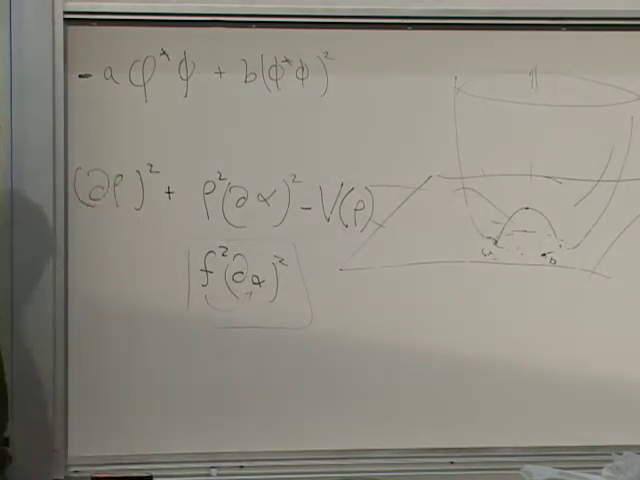
\includegraphics[width=0.88\textwidth]{lecture_07_figure_03.png}
\caption{Lagrangian của trường trong biến cực, hạng góc năng lượng thấp được đóng khung của nó, và thế năng phá vỡ đối xứng. Chuyển động theo bán kính leo lên thế năng; chuyển động theo góc đi dọc theo rãnh.}
\lectureframe{00:56:40}
\end{figure}

Đối với một kích thích năng lượng rất thấp, trường vẫn ở gần
\(\rho=f\). Khi đó
\begin{equation}
  \mathcal L_{\rm angular}
  \simeq f^2(\partial_\mu\alpha)(\partial^\mu\alpha).
\end{equation}
Định nghĩa trường góc được chuẩn hóa chính tắc, tùy theo quy ước dùng cho các thừa số \(1/2\), bằng
\begin{equation}
  \beta=\sqrt{2}\,f\alpha,
  \qquad
  \mathcal L_{\rm angular}
  =\frac12(\partial_\mu\beta)(\partial^\mu\beta).
  \label{eq:l07-goldstone-field}
\end{equation}
Không có hạng \(\beta^2\). Các lượng tử của trường góc này là không khối lượng. Chúng là các boson Goldstone.

Trường theo bán kính hành xử khác. Nếu dời \(\rho\) khỏi \(f\) đồng thời ở mọi nơi thì nó trở về, vượt quá, rồi dao động quanh rãnh. Nếu
\(\rho=f+h\), khai triển phương trình~\eqref{eq:l07-mexican-hat} cho
\begin{equation}
  V(f+h)=V(f)+\frac12m_h^2h^2+\cdots,
\end{equation}
nên \(h\) có khối lượng. Về mặt hình học, phương góc là phẳng còn phương bán kính là cong.

\begin{classroomqa}
\audiencequestion{Nếu trường bị lệch theo hướng xuyên tâm, liệu nó có đơn giản rơi trở lại xuống hay không, và sau đó điều gì xảy ra?\lecturetimestamp{00:57:10}}
\lecturerresponse{Nếu không có chuyển động góc, nó rơi về phía điểm cực tiểu, vượt quá điểm đó rồi dao động theo phương xuyên tâm. Một dao động đồng nhất có động lượng không gian bằng không nhưng tần số khác không; tần số đó là khối lượng của kích thích xuyên tâm. Ngược lại, một độ lệch góc đồng nhất đưa nó tới một chân không khác và không có lực phục hồi.}
\end{classroomqa}

Đây là nội dung của nguyên lý Goldstone trong ví dụ hiện tại: phá vỡ tự phát một đối xứng toàn cục liên tục sinh ra một mode không khối lượng cho mỗi phương phẳng độc lập của đa tạp chân không.
\editorialnote{Mệnh đề này giả sử các điều kiện thông thường của lý thuyết trường tương đối tính. Trong các hệ nhiều hạt phi tương đối tính, việc đếm số và quan hệ tán sắc của các mode Nambu--Goldstone có thể tinh tế hơn, nhưng kết luận ở giới hạn bước sóng dài của bài giảng vẫn là kết luận đúng cho mô hình \(U(1)\) tương đối tính này.}

\section{Sóng spin, dây và âm thanh}

Định lý thì trừu tượng, nhưng cơ chế của nó lại quen thuộc. Trong một sắt từ đẳng hướng, mọi spin có thể cùng quay mà không làm thay đổi năng lượng. Cho hướng đó biến thiên rất chậm trên toàn mẫu, ta thu được một sóng spin. Năng lượng phải trả cho nó triệt tiêu cùng với số sóng của nó, nên nó là mode Goldstone của đối xứng quay spin bị phá vỡ.

Một sợi dây đàn hồi dài cho ta một hình dung khác. Bỏ qua trọng lực và gắn hai đầu sao cho toàn bộ sợi dây có thể được tịnh tiến theo phương thẳng đứng. Một phép tịnh tiến thẳng đứng đồng nhất không tốn năng lượng. Nếu cho phép tịnh tiến đó biến thiên chậm dọc theo dây thì nó trở thành một sóng ngang bước sóng dài. Phép tác động đối xứng đồng nhất đã được nâng thành một biến dạng nhẹ phụ thuộc vị trí.

\begin{figure}[htbp]
\centering
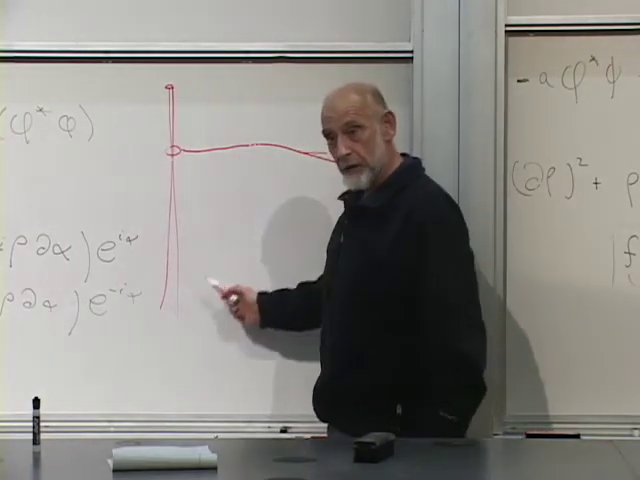
\includegraphics[width=0.68\textwidth]{lecture_07_figure_04.png}
\caption{Biên dạng sợi dây biến thiên chậm được vẽ trong phép tương tự mode Goldstone. Điểm vật lý là độ dốc nhỏ của một biến dạng bước sóng dài, chứ không phải vị trí theo phương thẳng đứng của đường cong.}
\lectureframe{01:04:19}
\end{figure}

\begin{classroomqa}
\audiencequestion{Sợi dây có thể mang năng lượng dao động trong khi có xung lượng bằng 0 không?\lecturetimestamp{01:04:41}}
\lecturerresponse{Cần phân biệt xung lượng cơ học theo phương thẳng đứng với xung lượng sóng dọc theo dây. Một sóng dừng có thể có tổng xung lượng bằng 0 vì nó là chồng chập của các mode có \(+k\) và \(-k\), trong khi vẫn mang năng lượng. Trong phép tương tự lý thuyết trường, xung lượng ám chỉ số sóng dọc theo trục; độ dời theo phương thẳng đứng đóng vai trò tọa độ nội tại của trường.}
\end{classroomqa}

Một lò xo slinky cho phiên bản dọc. Tịnh tiến toàn bộ lò xo slinky vô hạn lý tưởng hóa dọc theo trục của nó thì không có gì thay đổi. Tịnh tiến các phần lân cận những lượng hơi khác nhau thì kết quả là một sóng nén nhẹ. Trong chất rắn hoặc chất lưu, âm thanh bước sóng dài cũng tương tự như vậy, nảy sinh từ các độ dời tập thể và các biến thiên mật độ. Sóng spin, sóng ngang trên dây, và âm thanh không phải là cùng một kích thích vi mô, nhưng chúng chia sẻ khuôn mẫu quyết định: một phép tác động liên tục đồng nhất không tốn năng lượng, và phiên bản biến thiên chậm của nó trở thành một mode mềm.
\editorialnote{Trong tinh thể, các phonon âm học theo quy ước được mô tả là các mode Nambu--Goldstone của các phép tịnh tiến liên tục bị phá vỡ tự phát. Dây và lò xo slinky là những phép tương tự cơ học được dùng trong bài giảng để phơi bày cùng một cấu trúc năng lượng chỉ gồm đạo hàm.}

Thuật ngữ đủ quan trọng để có một câu đùa ngắn trên lớp: đây là các boson \emph{Goldstone}, được đặt theo tên Jeffrey Goldstone, chứ không phải boson chuẩn. Bài giảng lưu ý rằng Goldstone là bạn của Susskind, rồi chuyển sang chủ đề thực sự khác là bất biến chuẩn.

\section{Từ đối xứng pha toàn cục đến đối xứng chuẩn}

Đối xứng pha \(U(1)\) đã xuất hiện trong môn học này như là đối xứng gắn với sự bảo toàn điện tích. Các trường hạt mang điện là các trường phức, và việc nhân một trường như vậy với một pha chung không làm thay đổi lý thuyết toàn cục. Có thể dùng từ điện để trực giác hóa, dù điện tích ấy cũng có thể biểu diễn một số lượng tử \(U(1)\) khác. Photon thật sự là không khối lượng; đích đến cuối cùng là một trường kiểu photon như \(Z\) có khối lượng.

Câu hỏi mới là liệu
\begin{equation}
  \phi'(x)=e^{i\theta(x)}\phi(x)
  \label{eq:l07-local-u1}
\end{equation}
có thể là một đối xứng khi \(\theta\) biến thiên tùy ý trong không-thời gian hay không. Hàm \(\theta(x)\) là một tham số biến đổi, không phải một trường động lực bổ sung. Ta kiểm tra đề xuất này bằng cách lấy đạo hàm:
\begin{equation}
  \partial_\mu\phi'
  =e^{i\theta}
   \left[\partial_\mu\phi+i(\partial_\mu\theta)\phi\right].
  \label{eq:l07-local-derivative}
\end{equation}
Hạng phụ thêm đó vắng mặt khi \(\theta\) là hằng. Đối với trường liên hợp,
\begin{equation}
  \partial_\mu\phi^{*\prime}
  =e^{-i\theta}
   \left[\partial_\mu\phi^*-i(\partial_\mu\theta)\phi^*\right].
\end{equation}
Tích của chúng là
\begin{align}
  \partial_\mu\phi^{*\prime}\partial^\mu\phi'
  ={}&
  \partial_\mu\phi^*\partial^\mu\phi
  i\left(
      \phi\,\partial_\mu\phi^*
      -\phi^*\partial_\mu\phi
    \right)\partial^\mu\theta
  \nonumber\\
  &+\phi^*\phi\,
    \partial_\mu\theta\,\partial^\mu\theta.
  \label{eq:l07-local-failure}
\end{align}
Thế năng vẫn bất biến vì \(\phi^*\phi\) bất biến, nhưng hạng động năng thông thường thì không còn như vậy. Một đối xứng toàn cục không tự động trở thành một đối xứng cục bộ.

\begin{classroomqa}
\audiencequestion{Trong hình chiếc mũ Mexico, sự thất bại này có nghĩa là có những gợn nhô quanh rãnh tròn không?\lecturetimestamp{01:19:37}}
\lecturerresponse{Không. Thế năng vẫn có thể hoàn toàn phẳng theo phương góc. Cái giá phụ thêm đến từ các gradient khi pha khác nhau từ điểm không-thời gian này sang điểm không-thời gian khác. Đó không phải là sự nhấp nhô của rãnh; đó là hạng đạo hàm thông thường đang phát hiện sự biến thiên theo không gian.}
\end{classroomqa}

\subsection{Trường vectơ bù}

Các tương tác của photon, \(W\), \(Z\) và gluon trong tự nhiên được tổ chức bởi các đối xứng chuẩn cục bộ, chứ không chỉ bởi các phép biến đổi cứng. Để biến phép tác động pha cục bộ thành một đối xứng, hãy mở rộng lý thuyết bằng một trường bốn-vectơ \(A_\mu\). Trong điện từ học, \(A_0\) là thế vô hướng còn ba thành phần không gian tạo thành thế vectơ. Các đạo hàm của chúng tạo nên điện trường và từ trường.

Hãy chọn quy ước tự nhất quán
\begin{equation}
  \phi'=e^{i\theta}\phi,
  \qquad
  A'_\mu=A_\mu-\partial_\mu\theta,
  \qquad
  D_\mu=\partial_\mu+iA_\mu.
  \label{eq:l07-gauge-convention}
\end{equation}
Trên bảng, một dấu bị đổi trong lúc kiểm tra sự triệt tiêu; phương trình \eqref{eq:l07-gauge-convention} cố định đồng thời cả ba dấu. Hằng số ghép chuẩn và điện tích đã tạm thời được hấp thụ vào \(A_\mu\).
\editorialnote{Khi viết tường minh điện tích \(q\) và hằng số ghép \(g\), ta có thể viết \(D_\mu=\partial_\mu+igqA_\mu\) và
\(A'_\mu=A_\mu-(gq)^{-1}\partial_\mu\theta\). Bài giảng lược bỏ các hằng số này để sự triệt tiêu vẫn hiển lộ.}

Đối với trường liên hợp,
\begin{equation}
  D_\mu\phi^*=\partial_\mu\phi^*-iA_\mu\phi^*.
\end{equation}
Bây giờ
\begin{align}
  D'_\mu\phi'
  &=
  \left(\partial_\mu+iA'_\mu\right)e^{i\theta}\phi
  \nonumber\\
  &=
  e^{i\theta}
  \left[
    \partial_\mu\phi+i(\partial_\mu\theta)\phi
    +i(A_\mu-\partial_\mu\theta)\phi
  \right]
  \nonumber\\
  &=e^{i\theta}D_\mu\phi.
  \label{eq:l07-covariant-transform}
\end{align}
Đạo hàm không mong muốn của \(\theta\) được triệt tiêu bởi phép biến đổi của \(A_\mu\). Tương tự,
\begin{equation}
  D'_\mu\phi^{*\prime}=e^{-i\theta}D_\mu\phi^*.
\end{equation}
Tích của chúng là bất biến. Tính từ \emph{hiệp biến} có nghĩa là đạo hàm biến đổi theo cùng một cách đơn giản như chính trường đó.

\section{Động lực học của trường chuẩn}

Nếu chỉ đưa \(A_\mu\) vào để sửa một đạo hàm thì nó sẽ không có động lực học riêng. Cường độ trường bất biến chuẩn là
\begin{equation}
  F_{\mu\nu}
  =\partial_\mu A_\nu-\partial_\nu A_\mu.
  \label{eq:l07-field-strength}
\end{equation}
Nó là phản đối xứng, nên \(F_{\mu\mu}=0\). Các thành phần thời gian--không gian của nó chứa điện trường, còn các thành phần không gian--không gian chứa từ trường. Trong ngôn ngữ ba-vectơ quen thuộc, mật độ năng lượng điện từ tỉ lệ với \(\bm E^2+\bm B^2\), còn Lagrangian Lorentz tỉ lệ với \(\bm E^2-\bm B^2\), với các dấu phụ thuộc vào quy ước metric.

\begin{classroomqa}
\audiencequestion{Năng lượng và Lagrangian của trường điện từ là gì?\lecturetimestamp{01:33:20}}
\lecturerresponse{Năng lượng được xây dựng từ \(E^2+B^2\); Lagrangian dùng \(E^2-B^2\). Trong dạng hiệp biến, đại lượng sau được viết như một bội số theo quy ước của \(F_{\mu\nu}F^{\mu\nu}\). Tensor phản đối xứng đó là xoáy bốn chiều của thế vectơ.}
\end{classroomqa}

Bản thân cường độ trường cũng bất biến chuẩn:
\begin{align}
  F'_{\mu\nu}
  &=
  \partial_\mu(A_\nu-\partial_\nu\theta)
  -\partial_\nu(A_\mu-\partial_\mu\theta)
  \nonumber\\
  &=
  F_{\mu\nu}
  -\partial_\mu\partial_\nu\theta
  +\partial_\nu\partial_\mu\theta
  =F_{\mu\nu}.
  \label{eq:l07-field-strength-invariant}
\end{align}
Đẳng thức cuối cùng suy ra vì các đạo hàm riêng hỗn hợp thông thường giao hoán. Do đó, một Lagrangian bất biến chuẩn tiêu chuẩn là
\begin{equation}
  \boxed{
  \mathcal L
  =(D_\mu\phi)^*D^\mu\phi
  -V(\phi^*\phi)
  -\frac14F_{\mu\nu}F^{\mu\nu}}
  \label{eq:l07-scalar-qed}
\end{equation}
tùy theo quy ước về dấu và chuẩn hóa được chọn cho metric.

\begin{figure}[htbp]
\centering
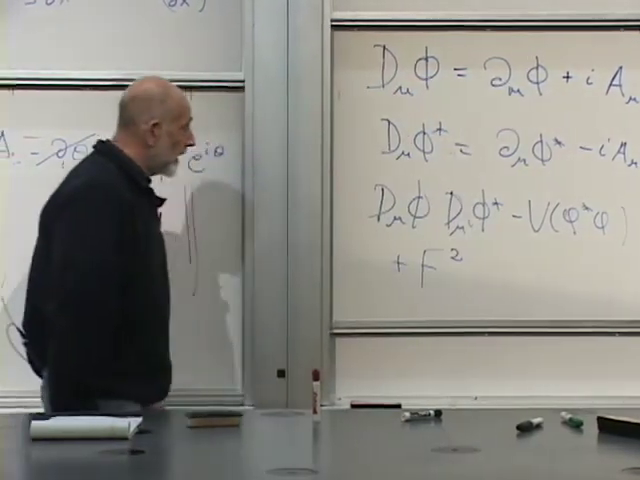
\includegraphics[width=0.84\textwidth]{lecture_07_figure_05.png}
\caption{Các đạo hàm hiệp biến và Lagrangian bất biến chuẩn được ghép lại trên bảng. Các thừa số số học được lược bỏ ở đó để cấu trúc biến đổi vẫn hiển lộ.}
\lectureframe{01:38:45}
\end{figure}

Cấu trúc này nâng một đối xứng toàn cục \(U(1)\) thành một đối xứng cục bộ, nhưng nó làm như vậy với cái giá---hay, về mặt vật lý, với món quà---là một trường vectơ mới. Trong ví dụ Abel, trường ấy chính là thế điện từ.

\begin{classroomqa}
\audiencequestion{Lagrangian ban đầu của ta dùng các đạo hàm thường. Vì sao chúng ta có quyền thay chúng bằng các đạo hàm hiệp biến và gọi kết quả là lý thuyết thực sự?\lecturetimestamp{01:42:55}}
\lecturerresponse{Chúng ta đang xây dựng một lý thuyết khác, được mở rộng: vật chất mang điện cộng với một trường chuẩn. Bất biến chuẩn cục bộ quyết định sự ghép của chúng. Lý thuyết lượng tử thu được là một cấu trúc toán học nhất quán và phù hợp với cách tự nhiên tổ chức photon và các trường chuẩn yếu. Chỉ riêng việc ghép một trường vectơ tương đối tính một cách không nhất quán có thể đưa vào các phân cực phi vật lý và sự vi phạm xác suất, vì vậy nguyên lý chuẩn không phải là một phép viết lại mang tính hình thức của lý thuyết vô hướng tự do cũ.}
\end{classroomqa}

\begin{classroomqa}
\audiencequestion{Vậy việc thêm trường mới chính là cơ sở biện minh cốt yếu cho sự sửa đổi này sao?\lecturetimestamp{01:44:57}}
\lecturerresponse{Đúng. Không có \(A_\mu\), đạo hàm của một trường sau phép quay cục bộ sẽ chứa một \(\partial_\mu\theta\) không bị triệt tiêu. Với \(A_\mu\) và quy luật biến đổi của nó, sự triệt tiêu diễn ra. Trong ngôn ngữ hình học, \(A_\mu\) là một liên hệ trên một bó sợi; phần toán học sâu hơn đó là có thật và hữu ích, nhưng phần đại số ở trên đã chứa điều cần thiết ở đây.}
\end{classroomqa}

\section{Vì sao khối lượng trần của boson chuẩn lại bị cấm}

Đối với một trường boson thông thường, khối lượng được biểu diễn bằng một số hạng bậc hai.
Ta rất dễ muốn thêm
\begin{equation}
  \Delta\mathcal L_{\rm Proca}
  =\frac12m^2A_\mu A^\mu.
  \label{eq:l07-proca}
\end{equation}
Nhưng dưới \(A_\mu\mapsto A_\mu-\partial_\mu\theta\),
\begin{equation}
  A'_\mu A^{\mu\prime}
  =
  A_\mu A^\mu
  -2A^\mu\partial_\mu\theta
  +\partial_\mu\theta\,\partial^\mu\theta,
\end{equation}
nên phương trình~\eqref{eq:l07-proca} không bất biến chuẩn. Ta không thể đưa một khối lượng vào lý thuyết chuẩn này bằng tay mà vẫn giữ đối xứng cục bộ của nó.

\begin{figure}[htbp]
\centering
\includegraphics[width=0.72\textwidth]{lecture_07_figure_07.png}
\caption{Số hạng khối lượng vectơ trần được đề xuất \(\tfrac12m^2A_\mu A^\mu\). Sự thất bại của nó dưới \(A_\mu\mapsto A_\mu-\partial_\mu\theta\) là chướng ngại dẫn tới cơ chế Higgs.}
\lectureframe{01:39:48}
\end{figure}

Đây là thế bế tắc bề ngoài. Bất biến chuẩn giải thích photon không khối lượng và bảo vệ lý thuyết khỏi các bậc tự do phi vật lý, nhưng \(W\) và \(Z\) lại có khối lượng. Lối thoát không thể là một khối lượng vectơ tường minh. Nó phải phát sinh từ các trường đã có mặt trong một Lagrangian bất biến chuẩn.

\begin{classroomqa}
\audiencequestion{Việc đưa bất biến chuẩn vào tự nó có sinh ra boson Goldstone không?\lecturetimestamp{01:45:51}}
\lecturerresponse{Không. Boson Goldstone xuất hiện khi một đối xứng \emph{toàn cục} liên tục bị phá vỡ tự phát, trước khi thế vectơ được đưa vào. Khi đối xứng trở thành cục bộ, một pha biến thiên có thể được bù bởi \(A_\mu\). Trong lý thuyết chuẩn bị phá vỡ, mode góc không còn là một hạt không khối lượng độc lập nữa; nó cung cấp phân cực bổ sung của trường vectơ nay đã có khối lượng. Bài giảng tiếp theo sẽ suy ra phát biểu đó chứ không chỉ đơn thuần tuyên bố nó.}
\end{classroomqa}

\begin{classroomqa}
\audiencequestion{Có điều nào trong số này giải thích được vì sao các con sông uốn khúc không?\lecturetimestamp{01:47:03}}
\lecturerresponse{Không biết có mối liên hệ trực tiếp nào ở đây. Các xoáy trong chất lỏng và thậm chí cả hình dạng của sinh vật chắc chắn có thể được mô tả bằng các phương pháp đối xứng, và ta không bao giờ nên ngạc nhiên khi bắt gặp các ý tưởng của lý thuyết trường ở những nơi bất ngờ, nhưng bài giảng này không hề nêu ra một lý thuyết chuẩn về sự uốn khúc của sông.}
\end{classroomqa}

\section{Điểm dừng của bài giảng}

Giờ đây ta đã có hai thành phần đã hứa ở phần đầu. Một đối xứng toàn cục liên tục với một đường tròn các chân không có một hướng góc phẳng, và sự biến thiên chậm của nó là một trường Goldstone không khối lượng. Một đối xứng cục bộ đòi hỏi một liên hệ chuẩn và các đạo hàm hiệp biến, đồng thời cấm khối lượng vectơ trực tiếp trong phương trình~\eqref{eq:l07-proca}.

Bước tiếp theo là dùng thế năng bị phá vỡ của phương trình~\eqref{eq:l07-mexican-hat} trong lý thuyết bất biến chuẩn của phương trình~\eqref{eq:l07-scalar-qed}. Khi đó hai điều xảy ra đồng thời: hạt Goldstone riêng rẽ biến mất khỏi phổ vật lý, và trường vectơ thu được khối lượng. Theo ngôn ngữ sư phạm thông dụng, đối xứng chuẩn bị phá vỡ tự phát; chính xác hơn, sự dư thừa chuẩn vẫn còn nguyên trong khi lý thuyết đi vào một pha Higgs với một kích thích vectơ có khối lượng.
\editorialnote{Một đối xứng chuẩn cục bộ là sự dư thừa trong mô tả chứ không phải một đối xứng vật lý thông thường tác dụng giữa các trạng thái quan sát được phân biệt. Bài giảng dùng lối nói tắt tiêu chuẩn về sự phá vỡ tự phát của đối xứng chuẩn. Phát biểu vật lý bất biến chuẩn là sự sắp xếp lại các bậc tự do trong pha Higgs.}

Đó là hiện tượng Higgs. Chúng ta vẫn chưa thực hiện nó. Bài giảng này đã làm phần việc khó hơn nhưng cần thiết là làm cho bài toán đủ chính xác để khi lời giải xuất hiện, nó sẽ là điều không thể tránh khỏi.